% Spotlight Reflex — Beamer Presentation
% Compile: pdflatex presentation.tex  (twice for cross-references)

\documentclass[aspectratio=169,10pt]{beamer}

% ── Theme ─────────────────────────────────────────────────────────────────────
\usetheme{metropolis}
\usepackage{appendixnumberbeamer}

% ── Packages ──────────────────────────────────────────────────────────────────
\usepackage{amsmath,amssymb}
\usepackage{graphicx}
\usepackage{booktabs}
\usepackage{colortbl}
\usepackage{xcolor}
\usepackage{tikz}
\usetikzlibrary{arrows.meta,positioning,fit,backgrounds}
\usepackage[expansion=false]{microtype}
\usepackage{hyperref}

% ── Colour palette ────────────────────────────────────────────────────────────
\definecolor{spotBlue}{HTML}{005F73}
\definecolor{spotTeal}{HTML}{0A9396}
\definecolor{spotGold}{HTML}{EE9B00}
\definecolor{spotRed}{HTML}{AE2012}
\definecolor{spotGreen}{HTML}{28A745}
\definecolor{spotPurple}{HTML}{6F42C1}
\definecolor{spotGray}{HTML}{6C757D}

\setbeamercolor{frametitle}{bg=spotBlue, fg=white}
\setbeamercolor{progress bar}{fg=spotGold}
\setbeamercolor{alerted text}{fg=spotGold}
\setbeamercolor{example text}{fg=spotTeal}

% ── Helpers ───────────────────────────────────────────────────────────────────
\newcommand{\highlight}[1]{\textcolor{spotGold}{\textbf{#1}}}
\newcommand{\good}[1]{\textcolor{spotGreen}{\textbf{#1}}}
\newcommand{\bad}[1]{\textcolor{spotRed}{\textbf{#1}}}
\newcommand{\code}[1]{\texttt{#1}}
\arrayrulecolor{spotBlue!40}

% ── Meta ──────────────────────────────────────────────────────────────────────
\title{Spotlight Reflex}
\subtitle{Minimal-Shot Autonomous Driving via Geometric World-State Reasoning}
\author{Alba Maria Tellez Fernandez}
\institute{amtellezfernandez@gmail.com · Waymo Open Dataset E2E Challenge}
\date{May 2026}

% ══════════════════════════════════════════════════════════════════════════════
\begin{document}
% ══════════════════════════════════════════════════════════════════════════════

\maketitle

\begin{frame}{Agenda}
  \tableofcontents[hideallsubsections]
\end{frame}

% ══════════════════════════════════════════════════════════════════════════════
\section{Motivation \& Claim}
% ══════════════════════════════════════════════════════════════════════════════

\begin{frame}{Who I Am \& What I Built}
  \begin{columns}[T]
    \begin{column}{0.52\textwidth}
      \textbf{Alba Maria Tellez Fernandez} · Lead AI, robotics logistics startup \\[0.4em]
      \textbf{Question behind this project:}
      \begin{itemize}\small
        \item Can a compact geometric representation replace learned scene priors?
        \item Does \emph{``avoid occupied space, preserve route''} generalise
              to geometry never seen in training?
      \end{itemize}
      \vspace{0.4em}
      \textbf{Two independent tracks — both from scratch:}
      \begin{itemize}\small
        \item \textbf{Spotlight Reflex} — closed-loop simulation policy
        \item \textbf{WOD-E2E harness} — trajectory selector on 479 real Waymo frames
      \end{itemize}
    \end{column}
    \begin{column}{0.45\textwidth}
      \begin{alertblock}{Main Claim}
        \small A driving policy that generalises to long-tail scenarios by reasoning from
        \textbf{occupancy, clearance, and route geometry} — not by memorising scenario
        labels or imitating average trajectories.
      \end{alertblock}
      \vspace{0.3em}
      \begin{block}{\small This is NOT}
        \begin{itemize}\small
          \item A production AV stack
          \item A strict zero-shot WOD-E2E claim
          \item A trained camera-perception system
        \end{itemize}
      \end{block}
    \end{column}
  \end{columns}
\end{frame}

\begin{frame}{The Problem — and the Failure}
  \begin{columns}[T]
    \begin{column}{0.50\textwidth}
      \textbf{Imitation learning} minimises:
      $\;\min_{f}\;\mathbb{E}_{(x,y)\sim\mathcal{D}}\bigl[\mathcal{L}(f(x),y)\bigr]$

      \vspace{0.3em}
      Works on the common driving distribution $\mathcal{D}$.
      Fails when $P_\text{test}\neq P_\text{train}$ — rare geometry,
      no fallback reasoning.

      \vspace{0.3em}
      \textbf{WOD-E2E} targets \textbf{11 scenario types} occurring
      $<$0.03\% of driving time: wrong-way actors, animals, debris,
      construction, cut-ins, cyclists.

      \vspace{0.3em}
      \begin{alertblock}{}
        \small Baseline: trajectory extrapolation only, no world-state reasoning.
        Drives directly into the actor.
      \end{alertblock}
    \end{column}
    \begin{column}{0.47\textwidth}
      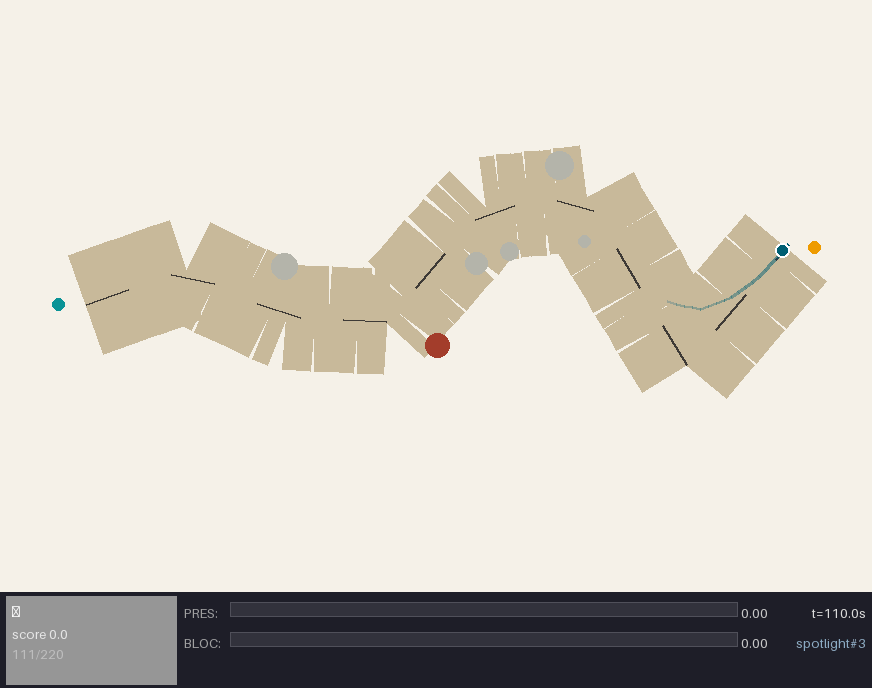
\includegraphics[width=\linewidth]{images/kf_baseline_spotlight.png}
      \vspace{0.1em}
      \small\textit{Wrong-way actor, night. Baseline has no awareness the path is occupied.}
    \end{column}
  \end{columns}
\end{frame}

% ══════════════════════════════════════════════════════════════════════════════
\section{Policy Architecture}
% ══════════════════════════════════════════════════════════════════════════════

\begin{frame}{Core Idea: Reason from Geometry, Not Memory}
  \begin{columns}[T]
    \begin{column}{0.50\textwidth}
      \textit{``A trajectory that avoids occupied space and respects route
      geometry is correct \textbf{regardless of what the obstacle is called}.''}

      \vspace{0.5em}
      \textbf{Formal invariance:} let $T$ be any relabelling of object identities,
      scenario names, or cluster tags that leaves occupancy $G$ and route $R$ unchanged.
      \[
        \boxed{M(s) = M(T(s)) \quad \forall\,s,\;\forall\,T}
      \]
      \texttt{"sheep"} $\to$ \texttt{"debris"} changes nothing.

      \vspace{0.3em}
      \small\textbf{Regression-tested:} a test suite relabels all objects in every
      scene and asserts maneuver, score, and reason are identical. Passes.
    \end{column}
    \begin{column}{0.47\textwidth}
      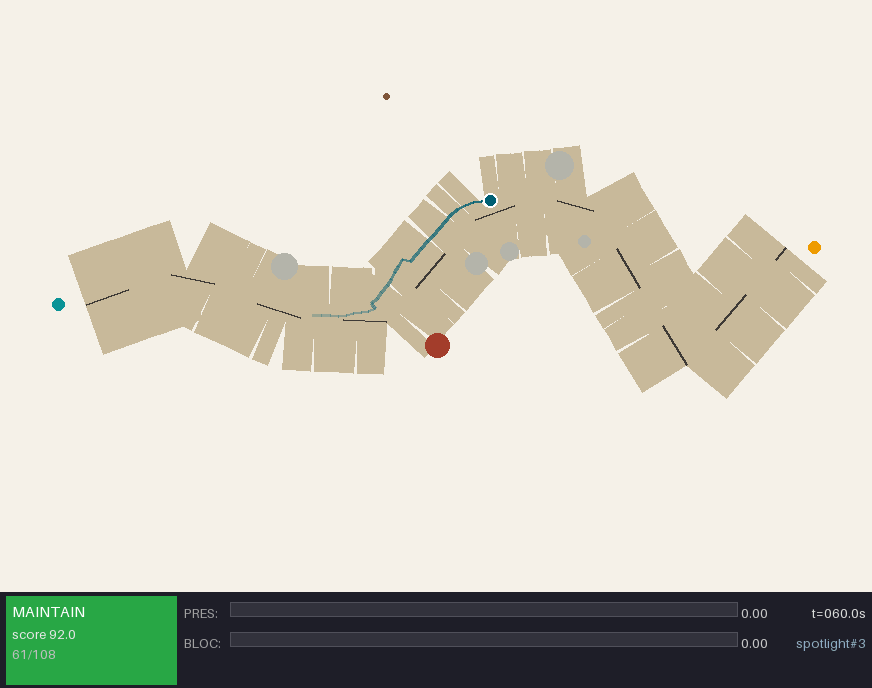
\includegraphics[width=\linewidth]{images/kf_spotlight_success.png}
      \vspace{0.1em}
      \small\textit{Same scenario, Spotlight Reflex: selects \code{evasive\_right},
      clears actor, returns to lane. Geometry resolved the decision.}
    \end{column}
  \end{columns}
\end{frame}

\begin{frame}{Six World-State Scalars}
  All signals computed from raw obstacle positions and route geometry.
  \textbf{Nothing is learned; nothing is scene-specific.}

  \vspace{0.4em}
  \begin{center}
  \small
  \begin{tabular}{llc}
    \toprule
    \textbf{Signal} & \textbf{Definition} & \textbf{Range} \\
    \midrule
    \code{obstacle\_pressure}      & $p = \mathrm{clip}\!\left(\tfrac{10-d_{\min}}{10},0,1\right)$
                                   & $[0,1]$ \\[4pt]
    \code{route\_blockage}         & fraction of forward corridor occupied & $[0,1]$ \\[4pt]
    \code{corridor\_blocked}       & hard blockage within stopping distance & bool \\[4pt]
    \code{left\_clearance}         & free lateral space to the left (m) & ${\geq}0$ \\[4pt]
    \code{right\_clearance}        & free lateral space to the right (m) & ${\geq}0$ \\[4pt]
    \code{preferred\_escape\_side} & $\arg\max(\mathrm{left},\mathrm{right})$ & L / R \\
    \bottomrule
  \end{tabular}
  \end{center}

  \vspace{0.3em}
  \small $d_{\min}$ = distance to nearest obstacle. Pressure = 1.0 at contact, 0 beyond 10\,m.
\end{frame}

\begin{frame}{Nine Maneuver Candidates}
  Each candidate: \textbf{20-point, 5\,s trajectory at 4\,Hz} via Hermite smoothstep.
  \textbf{Evasive maneuvers} apply the lateral offset early (first third) for fast separation.

  \vspace{0.3em}
  \begin{center}
  \footnotesize
  \begin{tabular}{p{2.5cm}p{3.0cm}cc}
    \toprule
    \textbf{Maneuver} & \textbf{Intent} & \textbf{Speed scale} & \textbf{Lateral offset} \\
    \midrule
    \code{stop}           & Emergency stop      & 0.00$\times$ & 0.0\,m \\
    \code{crawl}          & Very slow progress  & 0.15$\times$ & 0.0\,m \\
    \code{maintain}       & Hold current speed  & 1.00$\times$ & 0.0\,m \\
    \code{slow\_yield}    & Decelerate \& yield & 0.50$\times$ & 0.0\,m \\
    \code{nudge\_left}    & Minor left shift    & 0.80$\times$ & $+$0.9\,m \\
    \code{nudge\_right}   & Minor right shift   & 0.80$\times$ & $-$0.9\,m \\
    \code{evasive\_left}  & Strong left evasion & 0.70$\times$ & $+$2.2\,m \\
    \code{evasive\_right} & Strong right evasion& 0.70$\times$ & $-$2.2\,m \\
    \code{lane\_recover}  & Return to centre    & 0.90$\times$ & 0.0\,m \\
    \bottomrule
  \end{tabular}
  \end{center}
\end{frame}

\begin{frame}{Trust-Region Scoring \& Policy Architecture}
  \begin{columns}[T]
    \begin{column}{0.44\textwidth}
      \textbf{Speed-scaled tolerance:}
      \vspace{-0.2em}
      \[
        s(v)=\mathrm{clip}\!\left(\tfrac{v-1.4}{9.6},0,1\right)\!\times 0.5+0.5
      \]
      \vspace{-0.4em}
      \footnotesize
      \begin{tabular}{lcc}
        \toprule
        Horizon & Lateral & Longitudinal \\
        \midrule
        3\,s & $1.0{\times}s(v)$\,m & $4.0{\times}s(v)$\,m \\
        5\,s & $1.8{\times}s(v)$\,m & $7.2{\times}s(v)$\,m \\
        \bottomrule
      \end{tabular}
      \vspace{0.2em}
      \[
        S(\tau)=0.5\cdot\max_r\,\text{score}_{3s}+0.5\cdot\max_r\,\text{score}_{5s}
      \]
      \small Scores $\leq50$ = unsafe floor.
    \end{column}
    \begin{column}{0.53\textwidth}
      \small\textbf{How candidates are selected:}
      \begin{enumerate}\small
        \item Scene $\to$ compute 6 world-state scalars
        \item Reference rule engine maps scalars to expected maneuvers + scores
        \item Each of the 9 candidates is scored against references at 3\,s and 5\,s
        \item Highest combined score wins
      \end{enumerate}
      \vspace{0.3em}
      \small Every step emits a full \code{SpotlightSelection} log: maneuver,
      3\,s/5\,s scores, winning reference, decision reason, all scalar values.
      In AlpaSim: serialised as \code{reasoning\_text} JSON.
    \end{column}
  \end{columns}
\end{frame}

\begin{frame}{Policy Architecture — Decision Flow}
  \begin{center}
  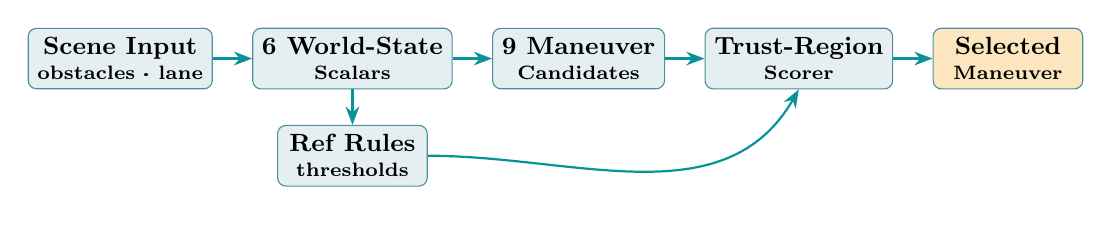
\begin{tikzpicture}[
    node distance=0.3cm and 0.5cm,
    box/.style={rectangle, rounded corners=3pt,
                draw=spotBlue!70, fill=spotBlue!10,
                minimum width=1.9cm, minimum height=0.72cm,
                font=\small\bfseries, align=center},
    arr/.style={-Stealth, thick, color=spotTeal}
  ]
    \node[box] (scene) {Scene Input\\[-2pt]\scriptsize obstacles · lane};
    \node[box, right=of scene]  (perc)  {6 World-State\\[-2pt]\scriptsize Scalars};
    \node[box, right=of perc]   (cands) {9 Maneuver\\[-2pt]\scriptsize Candidates};
    \node[box, below=0.45cm of perc] (refs) {Ref Rules\\[-2pt]\scriptsize thresholds};
    \node[box, right=of cands]  (score) {Trust-Region\\[-2pt]\scriptsize Scorer};
    \node[box, fill=spotGold!25, right=of score] (sel) {Selected\\[-2pt]\scriptsize Maneuver};

    \draw[arr] (scene) -- (perc);
    \draw[arr] (perc)  -- (cands);
    \draw[arr] (perc)  -- (refs);
    \draw[arr] (refs.east) to[out=0,in=240] (score.south);
    \draw[arr] (cands) -- (score);
    \draw[arr] (score) -- (sel);
  \end{tikzpicture}
  \end{center}

  \vspace{0.4em}
  \small
  \begin{columns}[T]
    \begin{column}{0.32\textwidth}
      \textbf{6 Scalars:} pressure, blockage, corridor blocked, left/right clearance,
      preferred escape side — all from raw geometry.
    \end{column}
    \begin{column}{0.32\textwidth}
      \textbf{Ref Rules:} world-state thresholds → expected maneuver + score
      (80–94 scale; $\leq50$ = unsafe).
    \end{column}
    \begin{column}{0.32\textwidth}
      \textbf{Scorer:} 3\,s + 5\,s horizons, speed-scaled tolerance.
      Full log emitted every step.
    \end{column}
  \end{columns}
\end{frame}

% ══════════════════════════════════════════════════════════════════════════════
\section{Simulation Results}
% ══════════════════════════════════════════════════════════════════════════════

\begin{frame}{The Simulator \& Compositional OOD}
  \begin{columns}[T]
    \begin{column}{0.54\textwidth}
      \textbf{Built from scratch — no Waymo or AlpaSim dependency.}
      \begin{itemize}\small
        \item Closed-loop 2D engine: ego + actors step simultaneously
        \item All 11 WOD-E2E scenario clusters implemented
        \item 8 actor behaviour models (linear, cut-in, swerve, erratic, wrong-way…)
        \item COMPASS composite benchmark (threshold 7.0/10)
      \end{itemize}
      \vspace{0.15em}
      \textbf{Compositional OOD:}
      $P(\text{topology},\text{hazard}) = P(\text{topology})\times P(\text{hazard})$\\[0.1em]
      \small 8 topologies $\times$ 11 hazards $\times$ 4 weather modes, sampled
      independently — a construction hazard can appear in a roundabout in fog.
    \end{column}
    \begin{column}{0.43\textwidth}
      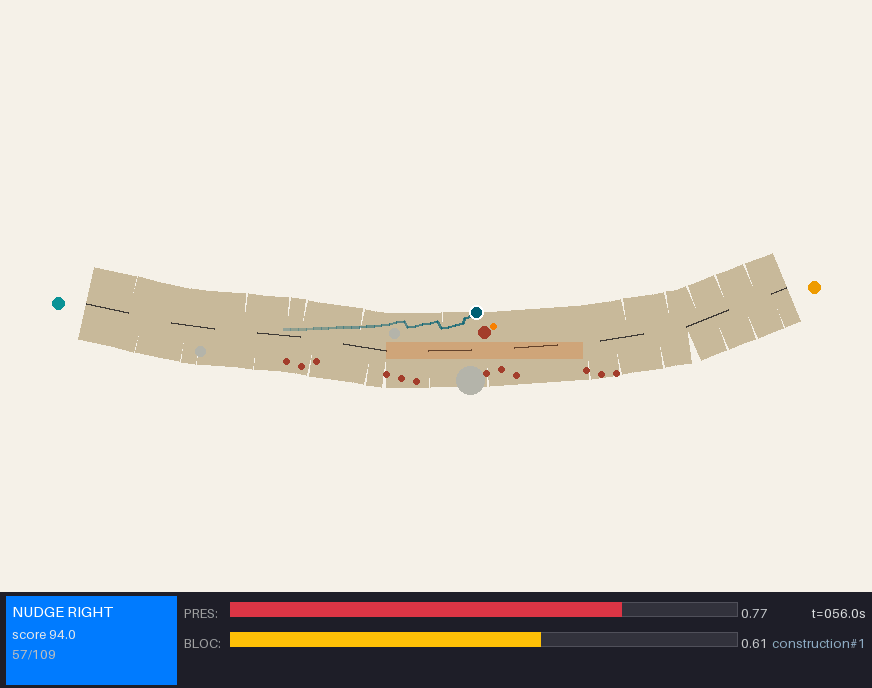
\includegraphics[width=\linewidth]{images/kf_construction.png}
      \vspace{0.15em}
      \small\textit{Construction zone — 5.2\,m corridor, cone field, lane closure.
      Policy: \code{nudge\_right}.}
    \end{column}
  \end{columns}
\end{frame}

\begin{frame}{Simulation Results}
  \textbf{Primary benchmark — 350 rollouts, seeds 1–10, deterministic:}

  \vspace{0.15em}
  \begin{columns}[T]
    \begin{column}{0.52\textwidth}
      \footnotesize
      \begin{tabular}{lrrr}
        \toprule
        \textbf{Suite} & \textbf{Runs} & \textbf{Coll.} & \textbf{Pass} \\
        \midrule
        WOD-style (11 clusters)    & 110 & \good{0} & \good{100\%} \\
        Compositional OOD          &  60 & \good{0} & \good{100\%} \\
        Adversarial (2–3 hazards)  &  60 & \good{0} & \good{100\%} \\
        Hidden holdout             &  60 & \good{0} & \good{100\%} \\
        Gauntlet (4h, 3.5\,m)     &  60 & \good{0} & 60\% \\
        \midrule
        \textbf{Total}             & \textbf{350} & \good{\textbf{0}} & \textbf{93.1\%} \\
        \bottomrule
      \end{tabular}\\[0.2em]
      \scriptsize COMPASS \highlight{9.137/10} · CI \highlight{[0.0, 0.0053]}
    \end{column}
    \begin{column}{0.45\textwidth}
      \textbf{Gauntlet — 420 matched scenarios:}\\[0.15em]
      \footnotesize
      \begin{tabular}{lcc}
        \toprule
        \textbf{Policy} & \textbf{Pass} & \textbf{Collision} \\
        \midrule
        Baseline            & 2.1\%  & \bad{20.5\%} \\
        \textbf{Spotlight Reflex} & \good{\textbf{57.6\%}} & \good{\textbf{7.9\%}} \\
        \bottomrule
      \end{tabular}\\[0.2em]
      \scriptsize 27$\times$ more passes · 2.6$\times$ fewer collisions.\\
      60\% gauntlet = failure boundary (4 hazards in 3.5\,m).
    \end{column}
  \end{columns}
\end{frame}

\begin{frame}{Scenarios \& AlpaSim Transfer}
  \begin{columns}[T]
    \begin{column}{0.31\textwidth}
      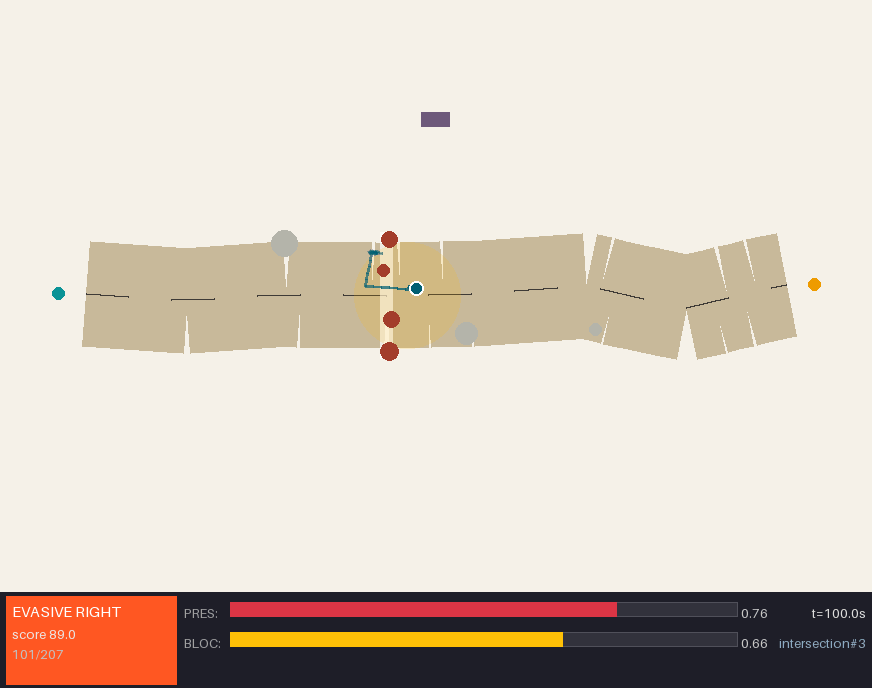
\includegraphics[width=\linewidth]{images/kf_intersection_stress.png}\\[0.2em]
      \small\textit{Intersection stress — two crossing actors, 207 steps. Zero collisions.}
    \end{column}
    \begin{column}{0.31\textwidth}
      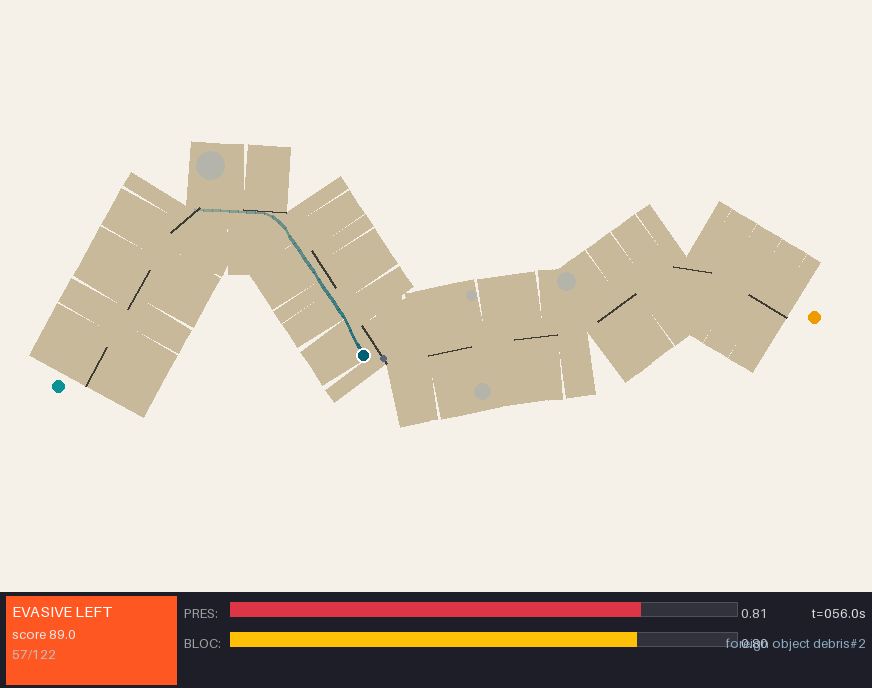
\includegraphics[width=\linewidth]{images/kf_fod.png}\\[0.2em]
      \small\textit{FOD — debris, primary lane blocked. \code{nudge\_right}.}
    \end{column}
    \begin{column}{0.35\textwidth}
      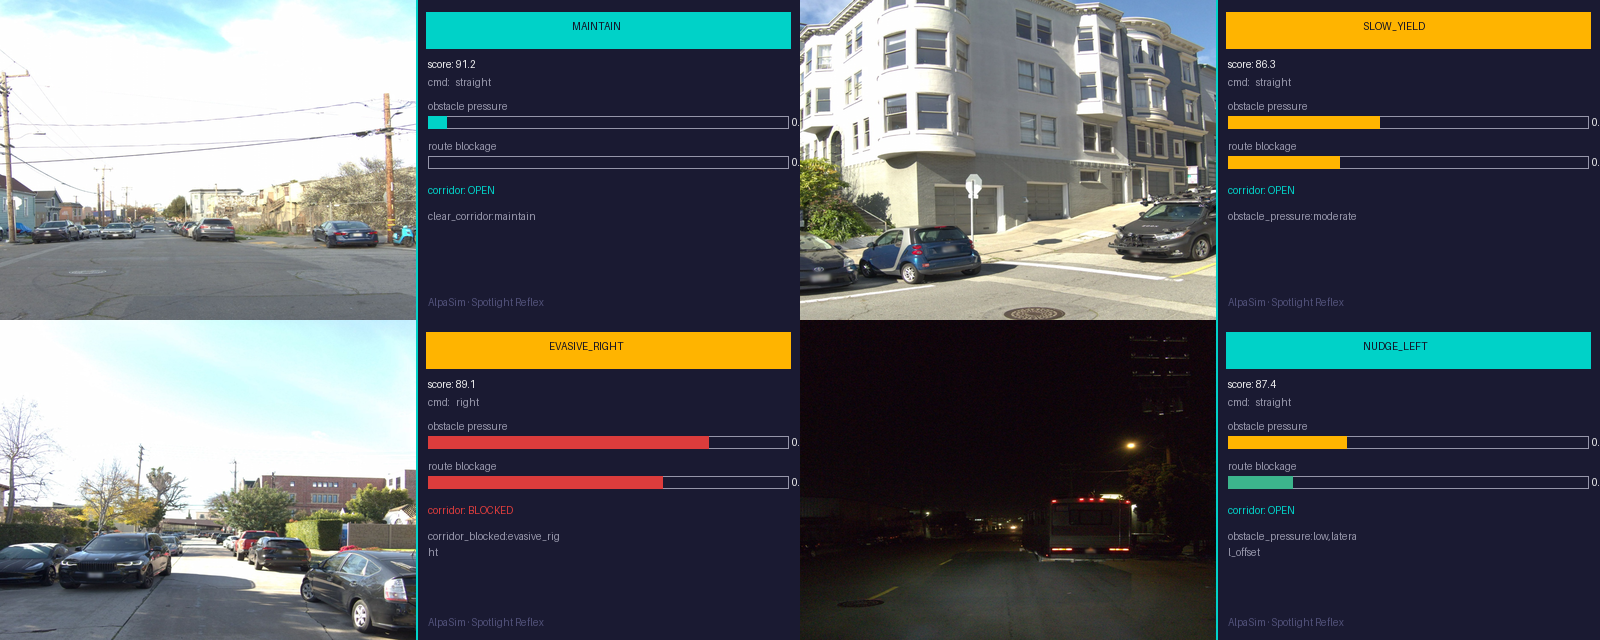
\includegraphics[width=\linewidth]{images/alpasim_reasoning_panel.png}\\[0.2em]
      \small\textit{AlpaSim — real Waymo camera + adapter output.}

      \vspace{0.25em}
      \small\textbf{4-channel adapter:}\\
      route, brightness, ego dynamics, hazards.\\
      Zero AlpaSim imports in the policy.\\[0.2em]
      \small\textbf{30 scenes:}\\
      \good{0.0} collision at fault\\
      0.42\,m dist.\ to GT traj.\\
      0.37 any-collision (others)
    \end{column}
  \end{columns}
\end{frame}

% ══════════════════════════════════════════════════════════════════════════════
\section{WOD-E2E Benchmark}
% ══════════════════════════════════════════════════════════════════════════════

\begin{frame}{WOD-E2E: Benchmark \& Selector Pipeline}
  \begin{columns}[T]
    \begin{column}{0.44\textwidth}
      \textbf{Waymo Open Dataset End-to-End:}
      \begin{itemize}\small
        \item 479 validation frames from real Waymo recordings
        \item Human raters: pairwise preferences between candidate trajectories
        \item \textbf{RFS} = how often the selected trajectory was preferred. Higher = better.
        \item \textbf{5-fold segment-grouped CV} — frames from the same driving segment
              stay together. Fold std $\approx0.19$, CI $\approx\pm0.17$.
      \end{itemize}
      \begin{alertblock}{\small Two backends — not interchangeable}
        \footnotesize Local: 7.131 · Official Waymo: 7.022.
        2-fold $\neq$ 5-fold — not comparable.
      \end{alertblock}
    \end{column}
    \begin{column}{0.53\textwidth}
      \small\textbf{Candidate sources:}
      \begin{itemize}\small
        \item \textbf{Kinematic:} const-vel, const-accel, heading change, stop
        \item \textbf{Ridge learned:} 31 trajectory features; target = gain vs baseline
        \item \textbf{Temporal:} ego-history trends; wins on 49\% of frames
      \end{itemize}
      \vspace{0.25em}
      \small\textbf{Selection:}\\
      HGB gate ranker ($\sim$137 features, 5-fold) picks best candidate.\\
      Direct policy overrides on $\sim$4\% of frames when confidence high.\\[0.3em]
      \footnotesize\textit{Frames → \{Kinematic | Ridge | Temporal\} → HGB Gate → Direct Policy → Output}
    \end{column}
  \end{columns}
\end{frame}

\begin{frame}{Visual Embeddings \& WOD-E2E Results}
  \begin{columns}[T]
    \begin{column}{0.45\textwidth}
      \textbf{Do image embeddings help the ranker?}

      \vspace{0.2em}
      \textbf{Cosmos} (NVIDIA): video autoencoder — 64-dim continuous latents.\\
      \textbf{InternVLA} (Shanghai AI Lab): ViT+LLM — 128-dim ViT output.
      Both failed under a linear (ridge) head. Non-linear model required.

      \vspace{0.1em}
      \footnotesize
      \begin{tabular}{p{2.3cm}p{1.8cm}r}
        \toprule
        \textbf{Config} & \textbf{Head} & \textbf{RFS} \\
        \midrule
        No embedding    & Ridge    & 7.803 \\
        Cosmos 64d      & Ridge    & $\approx$7.803 \\
        InternVLA 128d  & Ridge    & $\approx$7.803 \\
        RFF gate        & non-lin. & 7.834 \\
        \textbf{Cosmos 64d} & \textbf{GPU MLP} & \good{\textbf{7.845}} \\
        \bottomrule
      \end{tabular}
      \vspace{0.1em}\\
      \small Embeddings carry signal — only a non-linear model extracts it.
    \end{column}
    \begin{column}{0.51\textwidth}
      \textbf{Full results — 5-fold segment-grouped CV:}

      \vspace{0.2em}
      \small
      \begin{tabular}{p{3.8cm}cr}
        \toprule
        \textbf{Selector} & \textbf{Folds} & \textbf{RFS} \\
        \midrule
        Official Waymo baseline  & — & 7.022 \\
        Local CV baseline        & — & 7.131 \\
        Gate only                & 5 & 7.803 \\
        RFF direct policy        & 5 & 7.834 \\
        \textbf{GPU MLP + Cosmos 64d} & \textbf{5} & \good{\textbf{7.845}} \\
        HGB Optuna peak   & {\footnotesize 2 only} & 7.880 \\
        \midrule
        Oracle (perfect selector) & 5 & \highlight{9.264} \\
        \bottomrule
      \end{tabular}

      \vspace{0.2em}
      Champion: h=64 MLP, lr=0.003866, 4.2\% of frames, precision \highlight{0.60}\\[0.1em]
      \textbf{Oracle gap: \highlight{1.419 RFS}} — right candidate exists,\\
      \small selector can't identify it without visual scene information.
    \end{column}
  \end{columns}
\end{frame}

\begin{frame}{Honest Failures \& Next Steps}
  \begin{columns}[T]
    \begin{column}{0.50\textwidth}
      \textbf{What didn't work:}
      \vspace{0.15em}

      \footnotesize
      \begin{tabular}{p{2.3cm}p{4.3cm}}
        \toprule
        \textbf{Failure} & \textbf{Root cause} \\
        \midrule
        No camera perception &
          Sees only ego velocity, speed, accel, route intent.
          Cannot see debris or signals. \\[0.15em]
        Embeddings under linear head &
          Cosmos/InternVLA as ridge features — no gain.
          Signal requires a non-linear model. \\[0.15em]
        HGB Optuna 2-fold &
          7.880 under 2-fold; failed 5-fold.
          Optuna exploited fold structure. \\[0.15em]
        Turn calibration &
          GO\_RIGHT regret 2.063. Only 29 training frames for that intent. \\
        \bottomrule
      \end{tabular}
    \end{column}
    \begin{column}{0.47\textwidth}
      \textbf{Next steps:}
      \vspace{0.15em}

      \begin{enumerate}\small
        \item \textbf{Task-aligned encoder} (highest impact)\\
          \footnotesize Encoder fine-tuned on preference triplets (frame, win, loss).
          Expected: 0.5–1.5 RFS. Closes most of the 1.419 oracle gap.

        \item \textbf{Turn calibration}\\
          \footnotesize Stratified reweighting by intent class.
          GO\_LEFT: 1.753→1.614 already. GO\_RIGHT (2.063) next.

        \item \textbf{Test-set submission}\\
          \footnotesize Pipeline validated; 1,505 frames listed.
          Missing: test TFRecords (Waymo sign-in gated).

        \item \textbf{Physical deployment}\\
          \footnotesize Obstacle sensors + route command → Spotlight Reflex today.
          AlpaSim adapter is the real-sensor bridge template.
      \end{enumerate}
    \end{column}
  \end{columns}
\end{frame}

% ══════════════════════════════════════════════════════════════════════════════
\begin{frame}{Summary}
  \vspace{0.1em}
  \small
  \begin{tabular}{p{3.0cm}p{9.2cm}}
    \toprule
    \textbf{Core claim} &
      Geometric reasoning from 6 scalars generalises without training data for
      the scenario \\[0.2em]
    \textbf{Invariance} &
      $M(s)=M(T(s))$ — regression-tested: relabelling all objects → identical decisions \\[0.2em]
    \textbf{Simulator} &
      Built from scratch · 11 WOD clusters · compositional OOD · COMPASS 9.137/10 \\[0.2em]
    \textbf{Gauntlet} &
      57.6\% pass · 7.9\% collision vs baseline 2.1\% / 20.5\% · 27$\times$ improvement \\[0.2em]
    \textbf{WOD-E2E champion} &
      \textbf{7.845 RFS} (5-fold, GPU MLP + Cosmos 64d) · +0.714 vs local baseline \\[0.2em]
    \textbf{Oracle gap} &
      1.419 RFS — candidate pool is good; discriminator is the bottleneck \\[0.2em]
    \textbf{AlpaSim} &
      Same policy, sensor-realistic · 0.0 collision at fault · 0.42\,m to GT \\[0.2em]
    \textbf{Next step} &
      Task-aligned encoder fine-tuned on preference triplets \\
    \bottomrule
  \end{tabular}

  \vspace{0.2em}
  \begin{alertblock}{}
    \small Generalises from geometry, not memorised trajectories.
    The 1.419\,RFS oracle gap is recoverable with a preference-aligned visual encoder.
  \end{alertblock}
\end{frame}

\begin{frame}[standout]
  \Large Alba Maria Tellez Fernandez \\[0.5em]
  \normalsize\href{mailto:amtellezfernandez@gmail.com}{amtellezfernandez@gmail.com} \\[0.6em]
  \small
  \texttt{docs/simulation.md} · \texttt{docs/wod-e2e-system-walkthrough.md}
\end{frame}

% ══════════════════════════════════════════════════════════════════════════════
\appendix
% ══════════════════════════════════════════════════════════════════════════════

\begin{frame}{Appendix: Reference Rule Engine}
  Maps world-state threshold conditions to pseudo-rater references (name + score).

  \vspace{0.3em}
  \small
  \begin{tabular}{p{5.8cm}p{5.2cm}}
    \toprule
    \textbf{World condition} & \textbf{References (score)} \\
    \midrule
    Low pressure ($<0.25$), low uncertainty ($<0.45$), open corridor ($>0.35$)
      & \code{maintain} (92), lane centre (88) \\[0.2em]
    Moderate pressure ($>0.20$)
      & \code{slow\_yield} (86), best-side nudge (94), evasive (89) \\[0.2em]
    High uncertainty ($>0.55$)
      & \code{crawl} (90), \code{stop} (82) \\[0.2em]
    Lane offset $>0.3$\,m and speed $>0.5$\,m/s
      & \code{lane\_recover} (93) \\[0.2em]
    Default fallback
      & \code{maintain} (80), \code{slow\_yield} (76) \\
    \bottomrule
  \end{tabular}

  \vspace{0.2em}
  \small Scores 80–94 on a scale where $\leq50$ = unsafe rating.
\end{frame}

\begin{frame}{Appendix: Calibration Bias Audit}
  Regret = oracle RFS $-$ selected RFS. Where does the error live?

  \vspace{0.2em}
  \small
  \begin{tabular}{lcrrc}
    \toprule
    \textbf{Slice} & \textbf{$n$} & \textbf{Selected} & \textbf{Oracle} & \textbf{Regret} \\
    \midrule
    GO\_STRAIGHT & 427 & 7.959 & 9.336 & 1.377 \\
    GO\_LEFT     &  23 & 7.107 & 8.721 & \bad{1.614} \\
    GO\_RIGHT    &  29 & 6.574 & 8.638 & \bad{\textbf{2.063}} \\
    \midrule
    speed:fast   &  44 & 7.957 & 9.436 & 1.479 \\
    speed:slow   & 133 & 7.564 & 9.196 & \bad{1.632} \\
    speed:urban  & 136 & 8.132 & 9.416 & 1.285 \\
    \bottomrule
  \end{tabular}

  \vspace{0.2em}
  GO\_RIGHT ($n{=}29$) and GO\_LEFT ($n{=}23$) are rare — ranker is calibrated to
  GO\_STRAIGHT (89\% of frames). GO\_LEFT improved 1.753→1.614 with targeted changes.
  \textbf{Fix:} stratified loss reweighting by intent class.
\end{frame}

\begin{frame}{Appendix: RFF Derivation \& Optuna TPE}
  \begin{columns}[T]
    \begin{column}{0.50\textwidth}
      \textbf{Random Fourier Features} — approximate Gaussian kernel without $N{\times}N$ matrix:
      \begin{align*}
        \mathbf{W} &\sim \mathcal{N}(0,\sigma^{-2}I),\quad D{=}512,\;\sigma{=}7.858 \\
        \boldsymbol{\varphi}(\mathbf{x}) &=
          \sqrt{\tfrac{2}{D}}\cos(\mathbf{W}^\top\tilde{\mathbf{x}}+\mathbf{b}) \\
        \mathbb{E}[\boldsymbol{\varphi}^\top\boldsymbol{\varphi}'] &=
          \exp\!\left(-\tfrac{\|\mathbf{x}-\mathbf{x}'\|^2}{2\sigma^2}\right)
      \end{align*}
      Only 512-dim ridge weights are learned. RFS: 7.834, precision 0.41.
    \end{column}
    \begin{column}{0.47\textwidth}
      \textbf{Optuna TPE} — Bayesian optimisation:
      \begin{align*}
        \ell(x) &= P(x \mid \text{top-}p) \\
        g(x)    &= P(x \mid \text{bottom}) \\
        x_\text{next} &= \arg\max_x\;\tfrac{\ell(x)}{g(x)}
      \end{align*}
      \textbf{GPU MLP search (20 trials):}
      \begin{itemize}\small
        \item Best: trial\_0004 — $h{=}64$, lr=0.003866 → \good{7.845}
        \item Mean 20 trials: 7.769
        \item 1/20 beat the RFF baseline (7.834)
        \item With 479 frames + 5 folds, Optuna can exploit fold patterns
      \end{itemize}
    \end{column}
  \end{columns}
\end{frame}

\end{document}
